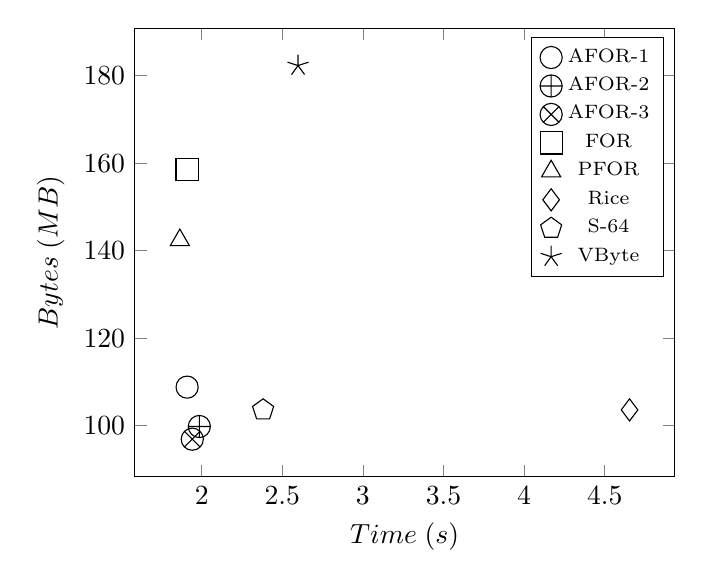
\begin{tikzpicture}
\begin{axis}[
scatter/classes={
	a={mark=o},
	b={mark=oplus},
	c={mark=otimes},
	d={mark=square},
	e={mark=triangle},
	f={mark=diamond},
	g={mark=pentagon},
	h={mark=star}
  },
  ylabel=$Bytes \; (MB)$,
  xlabel=$Time \; (s)$,
  mark options={scale=2},
  legend style={font=\scriptsize}
]

\addplot[scatter, only marks]
plot[scatter src=explicit symbolic]
coordinates {
(1.9096, 108.8) [a]
(1.9854, 99.8) [b]
(1.9415, 96.9) [c]
(1.9094, 158.5) [d]
(1.8644, 142.4) [e]
(4.654, 103.6) [f]
(2.381, 103.6) [g]
(2.5977, 182.3) [h]
};

\legend{AFOR-1, AFOR-2, AFOR-3, FOR, PFOR, Rice, S-64, VByte}

\end{axis}
\end{tikzpicture}